%%%%%%%%%%%%%%%%%%%%%%%%%%%%%%%%%%%%%%%%%%%%%%%%%%%%%%%%%%%%%%%%%%%%%%%%%%%%
% ICML-style draft.
% To compile with the official style, download icml2025.sty and
% icml2025.bst from the ICML author kit and uncomment the \usepackage line.
% As written this compiles standalone with the `article` class so the draft
% is portable; only the two-column ICML formatting is missing.
%%%%%%%%%%%%%%%%%%%%%%%%%%%%%%%%%%%%%%%%%%%%%%%%%%%%%%%%%%%%%%%%%%%%%%%%%%%%
\documentclass{article}
\usepackage{microtype}
\usepackage{graphicx}
\usepackage{booktabs}
\usepackage{multirow}
\usepackage{amsmath,amssymb}
\usepackage{hyperref}
\usepackage[margin=1in]{geometry}
\usepackage{xcolor}
\usepackage{caption}

% \usepackage{icml2025}   % <- swap in for the official two-column format

\title{Try Again, Don't Look Back:\\
Blind Resampling Outperforms Self-Repair in Small Code Models}
\author{Yuvraj Verma}
\date{}

\newcommand{\pass}{\mathrm{pass}@1}

\begin{document}
\maketitle

\begin{abstract}
Self-repair---showing a code model its failed attempt and asking it to fix the
problem---is a standard component of agentic coding systems, and is almost
always evaluated against a \emph{no-repair} baseline. We argue this is the
wrong comparison. Across three model scales
($1.5$B/$3$B/$7$B, Qwen2.5-Coder) on MBPP+, we run a pre-registered,
placebo-controlled ablation in which each retry receives nothing, a
content-free failure notice, real execution feedback, or feedback plus verbal
self-reflection, all at a matched iteration budget and against a
\emph{blind-resampling} control. Blind resampling wins at every scale, using
$2.5$--$5.5\times$ fewer tokens; conditioning on the model's own failed
attempt costs $6.1$ points at $1.5$B ($p{=}0.006$), and execution-feedback
\emph{content} adds nothing over a content-free placebo anywhere. We identify
the mechanism as \textbf{anchoring}: shown its own code, the model regenerates
a near-identical solution $33$--$68\%$ of the time versus $2$--$14\%$ when
resampling blind. Two further experiments sharpen the claim: retrieved
other-task exemplars have no effect in either direction (bounded to
$\pm3.5$ pp), isolating the penalty as specific to self-conditioning; and
verbal reflection loosens the anchor most yet still fails to pay for itself,
with anchoring rank predicting performance rank exactly. The methodological
lesson generalizes: for any prompt-augmenting capability, the control must be
an equally expensive but uninformative alternative, not the absence of the
capability.
\end{abstract}

\section{Introduction}
\label{sec:intro}

Iterative self-repair is widely used in code agents: after a generated program
fails its tests, the model is shown the program and (often) the failing output
and asked to correct it \citep{shinn2023reflexion,madaan2023selfrefine,
olausson2023selfrepair}. The near-universal way to justify this loop is to
compare it against a single-shot, no-repair baseline and report the
improvement. Such comparisons are confounded: repair spends additional
generation budget, and \emph{any} additional attempt---informative or
not---raises the chance of success under stochastic decoding. The reported
gain therefore conflates two effects: the value of the feedback content, and
the value of simply trying again.

We remove this confound with a placebo-controlled design and a
\emph{blind-resampling} control that spends the same iteration budget with no
feedback at all. Our central finding is counter-intuitive and robust: in the
$1.5$B--$7$B regime, self-repair is \emph{worse} than blind resampling, on
both accuracy and cost. We trace this to \textbf{anchoring}---a prompt
containing the failed attempt biases the model toward minor edits of a wrong
approach, whereas a fresh draw can explore a different region of the solution
space. We measure anchoring directly as inter-attempt code similarity, show it
predicts the ordering of every own-output condition, and show via a memory
experiment that it is specific to conditioning on one's \emph{own} output.

\paragraph{Contributions.}
\begin{enumerate}
  \item A pre-registered, placebo-controlled decomposition of the self-repair
  feedback packet at three model scales, with blind resampling as the control
  that prior work omits (\S\ref{sec:repair}).
  \item The finding that self-repair is worse than retrying below $7$B, on both
  accuracy and token cost.
  \item A mechanism---anchoring---measured from inter-attempt similarity, which
  explains both the scale trend and the ordering of all own-output conditions
  (\S\ref{sec:anchoring}).
  \item A null result on retrieved experience that isolates the mechanism as
  self-specific rather than a generic long-prompt effect (\S\ref{sec:memory}).
  \item A test of whether verbal reflection escapes the mechanism: it loosens
  the anchor measurably but not enough to pay for itself (\S\ref{sec:reflect}).
  \item A fully reproducible harness that runs on a single $6$\,GB consumer
  GPU, with every experiment pre-registered before running.
\end{enumerate}

\section{Related Work}
\label{sec:related}

\paragraph{Self-repair and self-refinement.}
Reflexion \citep{shinn2023reflexion} and Self-Refine
\citep{madaan2023selfrefine} popularized verbal self-feedback loops.
\citet{olausson2023selfrepair} question whether self-repair is a ``silver
bullet'' and note that gains often shrink under fair budget accounting; we
extend that scrutiny with an explicit placebo and blind-resampling control
across scale, and identify a mechanism. Recent placebo-style decompositions on
sub-$1.5$B models report that feedback content beats generic placebos; we find
that contrast indistinguishable from zero once blind resampling is included.

\paragraph{Execution feedback in agents.}
Agent-computer interfaces \citep{yang2024sweagent} and benchmark suites
\citep{jimenez2024swebench} make execution feedback central to modern coding
agents; Agentless \citep{xia2024agentless} shows a fixed
localize--repair--validate pipeline is competitive. A parallel line finds that
for frontier agents on repository-level tasks, prohibiting execution costs
little while saving substantial tokens. Our $7$B results are consistent with
that regime, while our smaller scales reveal active harm.

\paragraph{Retrieval and experience.}
Retrieval-augmented few-shot prompting \citep{liu2024rag4code} and
experience-driven issue resolution \citep{zhang2024codagentexp} report gains
from relevant exemplars. We find no such effect for lexically retrieved
exemplars in small-model code synthesis, and use the null to isolate our
mechanism. Self-improvement systems such as the Darwin G{\"o}del Machine
\citep{zhang2025dgm} motivate the broader agenda but operate at compute scales
outside our envelope.

\paragraph{Evaluation.}
We use $\pass$ \citep{chen2021codex} on the EvalPlus suites
\citep{liu2023evalplus}, which augment HumanEval \citep{chen2021codex} and MBPP
\citep{austin2021mbpp} with $35$--$80\times$ more tests. Statistics follow
McNemar's exact test \citep{mcnemar1947}, the bootstrap
\citep{efron1979bootstrap}, Wilson intervals \citep{wilson1927}, and Holm
correction \citep{holm1979}; retrieval uses BM25 \citep{robertson2009bm25}.

\section{Method}
\label{sec:method}

\paragraph{Models and benchmark.}
We evaluate Qwen2.5-Coder \citep{hui2024qwencoder} at $1.5$B, $3$B and $7$B
(Instruct, $Q4\_K\_M$), served locally. Our primary benchmark is MBPP+
($378$ tasks); HumanEval+ ($164$) is reported as secondary and is underpowered
here ($32$--$75$ failing tasks per cell versus $110$--$164$ on MBPP+). EvalPlus
ships inputs and a canonical oracle rather than expected outputs, so we score
by differential testing: a candidate passes an input iff it agrees with the
reference solution on that input.

\paragraph{Conditions.}
The baseline is greedy single-shot generation. On failure, a repair attempt
appends one of the following to the original instruction; the conditions differ
\emph{only} in that suffix:
\begin{itemize}
  \item \textbf{resample}: nothing (identical to the first prompt)---isolates
  the value of another draw.
  \item \textbf{placebo}: the failed code $+$ a content-free notice
  (``your solution was incorrect'')---isolates the value of seeing one's
  attempt.
  \item \textbf{feedback}: the failed code $+$ real execution output (failing
  input, expected, actual)---isolates the value of the facts.
  \item \textbf{reflect}: as feedback, plus ``first diagnose the failure, then
  fix''---isolates verbal reasoning.
\end{itemize}
Reading \textsf{resample}$\to$\textsf{placebo}$\to$\textsf{feedback}
decomposes the feedback packet; \textsf{feedback}$\to$\textsf{reflect} adds
reasoning.

\paragraph{Decoding.}
Retries sample at temperature $0.8$, identically across conditions; only the
shared $k{=}0$ point is greedy. This is forced: at temperature $0$ the model
returns a byte-identical solution every iteration, which would reduce
\textsf{resample} to a no-op and flatten every curve by construction.

\paragraph{Nested $k$.}
A single $k_{\max}{=}8$ trajectory records a verdict after every iteration, so
$\pass$ for all $k\le 8$ is read from one run:
\[
\pass(k) \;=\; \frac{1}{N}\sum_{i=1}^{N}
  \mathbb{1}\!\left[\exists\, j \le k : \text{attempt } j \text{ of task } i
  \text{ passes}\right].
\]
This is cheaper than independent runs per $k$ and better paired: the $k{=}1$
and $k{=}8$ arms share the identical trajectory prefix. All repair arms start
from the \emph{same} baseline run, so pairing between baseline and arm is exact
rather than statistical, and a solved task consumes no further attempts.

\paragraph{Statistics.}
For each paired contrast we report McNemar's exact test on discordant pairs
\citep{mcnemar1947} and a task-level bootstrap CI on the difference
\citep{efron1979bootstrap}, with Holm correction \citep{holm1979} across the
primary contrasts ($\alpha{=}0.05$). Pass rates carry Wilson intervals
\citep{wilson1927}. Every hypothesis, decision rule, and falsification
criterion was registered before the corresponding run.

\section{Self-Repair Is Worse Than Retrying}
\label{sec:repair}

\begin{figure*}[t]
  \centering
  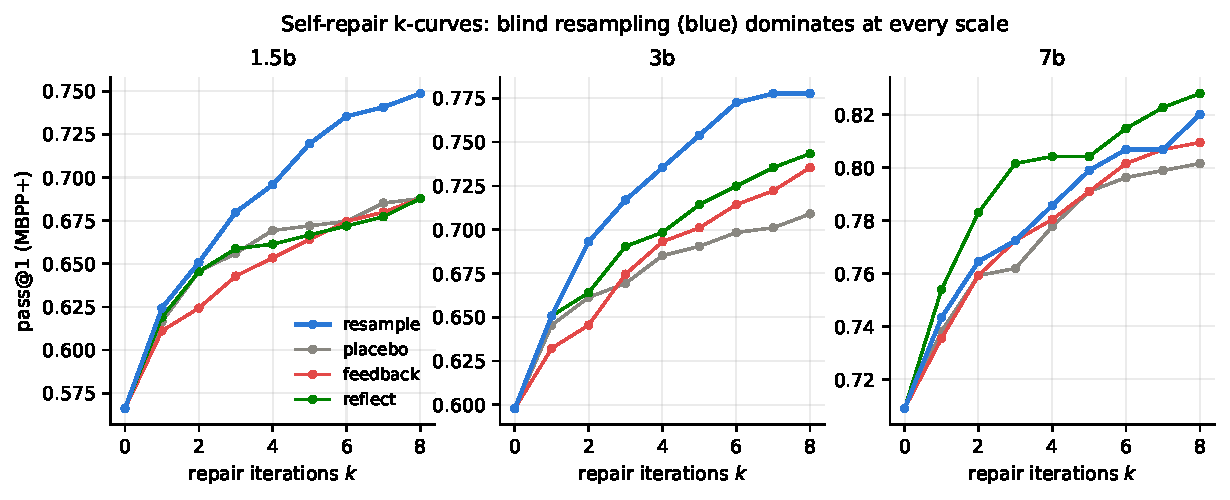
\includegraphics[width=\textwidth]{figures/fig1_kcurves.pdf}
  \caption{$\pass$ on MBPP+ as a function of repair iterations $k$. Blind
  resampling (blue) dominates the own-output conditions at $1.5$B and $3$B; at
  $7$B the ordering compresses and reflection (green) edges ahead. Curves are
  nested from a single $k{=}8$ trajectory per arm.}
  \label{fig:kcurves}
\end{figure*}

Figure~\ref{fig:kcurves} shows the $k$-curves. At $k{=}8$ (Table~\ref{tab:main}),
blind resampling attains the highest $\pass$ at $1.5$B and $3$B and is
statistically tied at $7$B, while every own-output condition is at or below it
(Figure~\ref{fig:forest}). The two pre-registered hypotheses on feedback are
refuted:
\begin{itemize}
  \item \textbf{Feedback content does not help}: $\textsf{feedback}-\textsf{placebo}$
  is $+0.000/+0.026/+0.008$ across scale, none significant.
  \item \textbf{Seeing one's own code hurts}: $\textsf{placebo}-\textsf{resample}$
  is $-0.061$ ($p{=}0.006$) at $1.5$B and $-0.069$ ($p{<}0.001$) at $3$B.
\end{itemize}

\begin{table}[t]
  \centering
  \small
  \caption{$\pass$ on MBPP+ at $k{=}8$ (Wilson $95\%$ CI), with output-token
  cost. Best per model in \textbf{bold}. Blind resampling is best or tied
  everywhere, at the lowest cost.}
  \label{tab:main}
  \begin{tabular}{llcc}
    \toprule
    Model & Condition & $\pass$ & Tokens \\
    \midrule
    \multirow{4}{*}{$1.5$B}
      & resample  & \textbf{0.749} [.72,.79] & \textbf{63k} \\
      & placebo   & 0.688 [.64,.73] & 90k \\
      & feedback  & 0.688 [.64,.73] & 129k \\
      & reflect   & 0.688 [.64,.73] & 345k \\
    \midrule
    \multirow{4}{*}{$3$B}
      & resample  & \textbf{0.778} [.73,.82] & \textbf{76k} \\
      & placebo   & 0.709 [.66,.75] & 89k \\
      & feedback  & 0.735 [.69,.78] & 84k \\
      & reflect   & 0.743 [.70,.79] & 284k \\
    \midrule
    \multirow{4}{*}{$7$B}
      & resample  & 0.820 [.78,.86] & \textbf{49k} \\
      & placebo   & 0.802 [.76,.84] & 59k \\
      & feedback  & 0.810 [.77,.85] & 55k \\
      & reflect   & \textbf{0.828} [.79,.86] & 122k \\
    \bottomrule
  \end{tabular}
\end{table}

\begin{figure}[t]
  \centering
  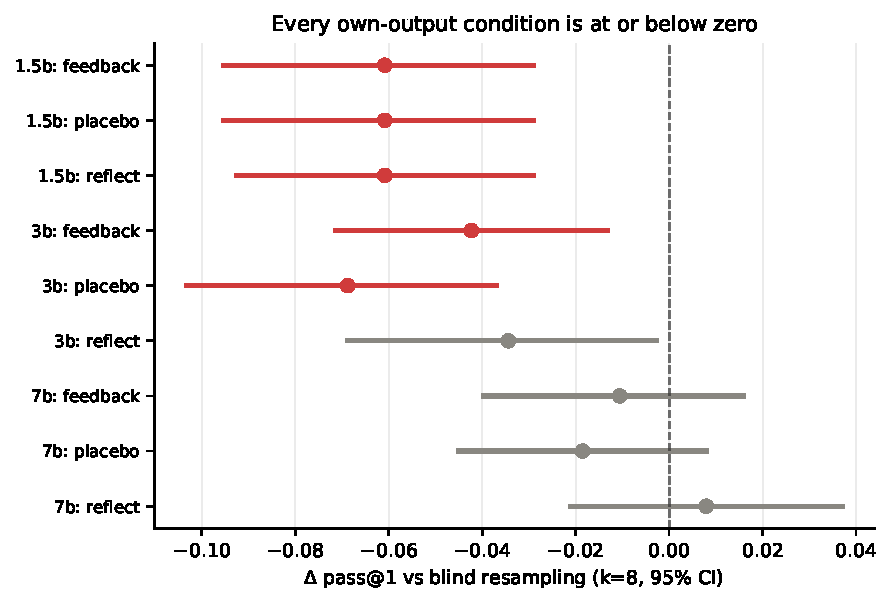
\includegraphics[width=\columnwidth]{figures/fig2_forest.pdf}
  \caption{Paired $\Delta\pass$ versus blind resampling at $k{=}8$
  ($95\%$ bootstrap CI). Red: significant loss after Holm correction; grey:
  n.s. No own-output condition significantly beats resampling at any scale.}
  \label{fig:forest}
\end{figure}

\paragraph{Cost.}
Blind resampling attains the best accuracy at the \emph{lowest} token cost
(Figure~\ref{fig:pareto}); it exits early more often because it succeeds more.
There is no accuracy/cost trade-off to navigate: the own-output conditions are
Pareto-dominated.

\paragraph{The knee.}
Marginal gain decays quickly: $46$--$53\%$ of all attainable improvement
arrives by $k{=}2$ at every scale, and marginal gains reach $\approx 0$ by
$k{=}7$. Iteration budgets beyond $k\!\approx\!2$ buy little regardless of
condition.

\begin{figure}[t]
  \centering
  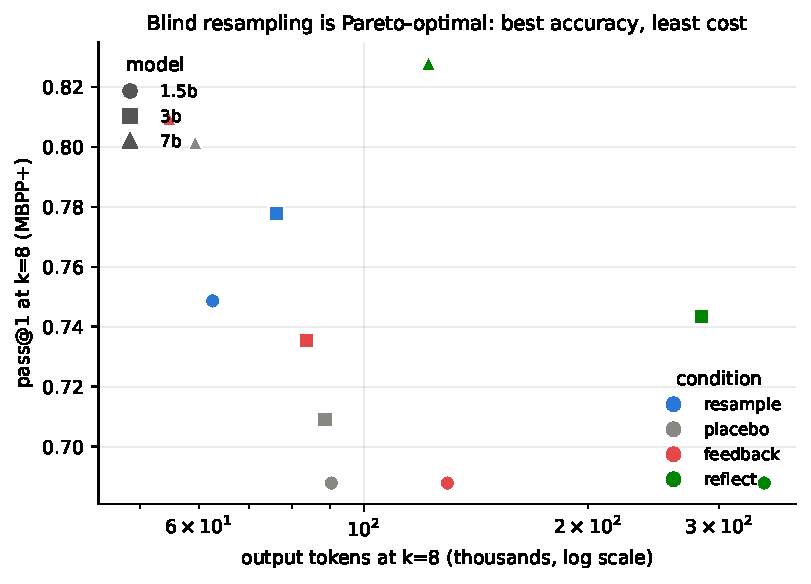
\includegraphics[width=0.92\columnwidth]{figures/fig4_pareto.pdf}
  \caption{$\pass$ at $k{=}8$ versus output tokens (log scale). Blind
  resampling (blue) is Pareto-optimal at every scale.}
  \label{fig:pareto}
\end{figure}

\section{The Mechanism Is Anchoring}
\label{sec:anchoring}

We hypothesized before measuring that conditioning on the failed attempt biases
the model toward minor edits. We test this by the mean similarity between
consecutive attempts, using \texttt{difflib}'s ratio on extracted code
(Figure~\ref{fig:anchoring}).

\begin{figure}[t]
  \centering
  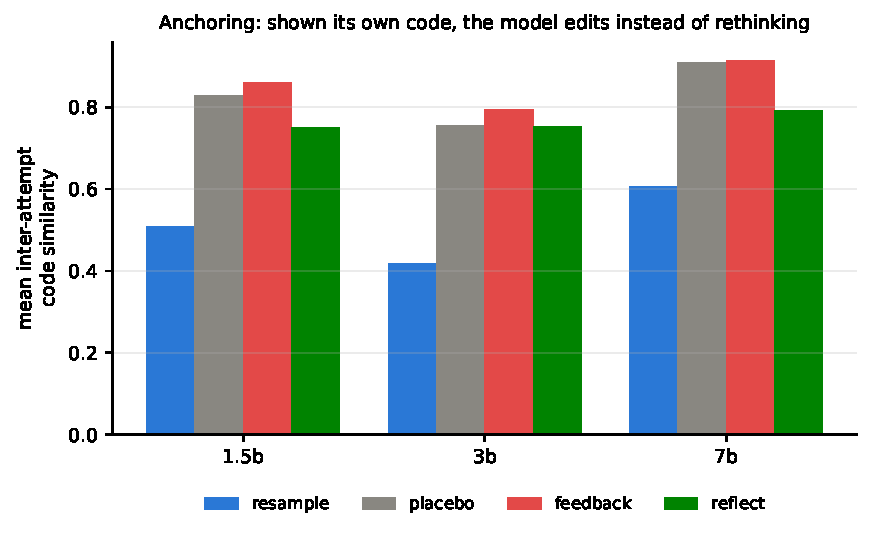
\includegraphics[width=\columnwidth]{figures/fig3_anchoring.pdf}
  \caption{Mean inter-attempt code similarity. Shown its own code
  (placebo/feedback/reflect), the model regenerates near-identical solutions
  far more often than when resampling blind.}
  \label{fig:anchoring}
\end{figure}

The effect is large and consistent: similarity rises by $+0.30$ to $+0.38$
relative to blind resampling at every scale, and near-identical regeneration
($>0.95$) rises from $2$--$14\%$ to $33$--$68\%$. This also explains the scale
trend the hypothesis did not anticipate. Anchoring \emph{strength} is roughly
constant across scale, but its \emph{cost} falls: a larger model's failed first
attempt is a better thing to anchor on. The shrinking penalty at $7$B is not
feedback becoming useful; it is anchoring becoming cheap.

\paragraph{Ordering.}
Among the three own-output conditions, anchoring rank predicts performance rank
exactly and inversely (Figure~\ref{fig:ordering}): the most-anchored condition
performs worst and the least-anchored best. A mechanism that predicts an
ordering it was not fitted to is stronger evidence than the headline contrast
alone.

\begin{figure}[t]
  \centering
  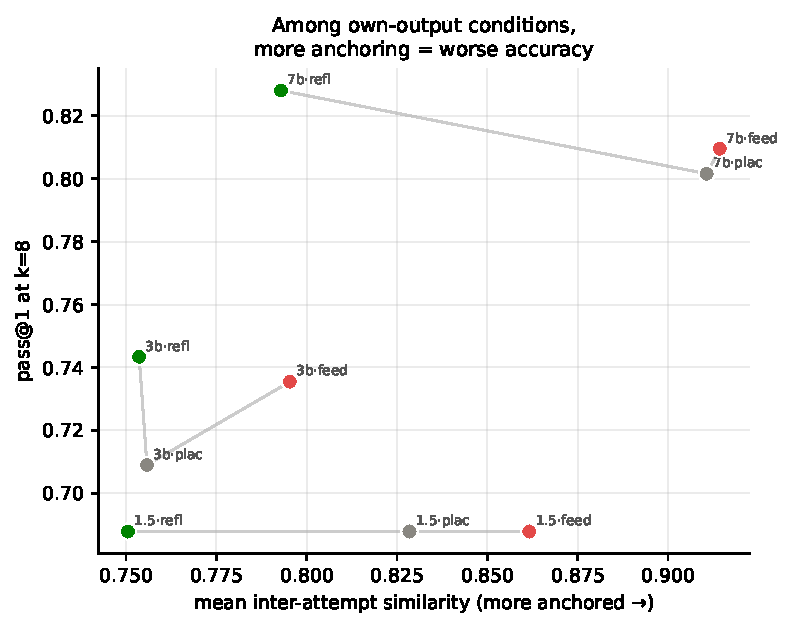
\includegraphics[width=0.88\columnwidth]{figures/fig5_ordering.pdf}
  \caption{Within each model, more inter-attempt similarity (more anchoring)
  corresponds to lower $\pass$. Lines connect the three own-output conditions
  per model.}
  \label{fig:ordering}
\end{figure}

\section{Retrieved Experience Does Nothing---Informatively}
\label{sec:memory}

If the repair penalty were a generic ``long prompts distract small models''
effect, then adding \emph{any} code to the context should hurt. We test this by
prepending $k{=}2$ solved exemplars, drawn either at random or by BM25
relevance, from the model's own past solutions (leave-one-out; a task never
retrieves itself). A leakage audit run before the experiment found only
$1.2$--$1.7\%$ of exemplars exceed $0.8$ similarity to the gold solution.

\begin{table}[t]
  \centering
  \small
  \caption{$\pass$ on MBPP+ with retrieved experience. All nine paired
  contrasts are non-significant after Holm correction; effects are bounded to
  $\pm3.5$ pp.}
  \label{tab:memory}
  \begin{tabular}{lccc}
    \toprule
    Model & none & random & retrieved \\
    \midrule
    $1.5$B & 0.566 & 0.542 & 0.542 \\
    $3$B   & 0.598 & 0.595 & 0.606 \\
    $7$B   & 0.709 & 0.728 & 0.696 \\
    \bottomrule
  \end{tabular}
\end{table}

The result is a clean null (Table~\ref{tab:memory}). Placed beside
\S\ref{sec:repair}, it is decisive: both interventions add comparable code to
the context, yet the \emph{own failed attempt} costs $6.1$ pp while
\emph{other tasks' solved code} costs nothing. The damage is specific to
self-conditioning---exactly what anchoring predicts and a context-dilution
account does not. We note this contradicts retrieval-augmented few-shot results
on classification tasks, where exemplars teach an output convention; MBPP+
specifies its format already, and our retriever is lexical.

\section{Reflection Loosens the Anchor but Cannot Pay for It}
\label{sec:reflect}

Reflexion-style reasoning \citep{shinn2023reflexion} is the natural candidate
to break the anchor: diagnosing \emph{why} an approach failed could license
abandoning it. It does, partially. Reflection is the only own-output condition
that meaningfully reduces anchoring---inter-attempt similarity drops by
$0.11$/$0.04$/$0.12$ relative to feedback, and near-identical regeneration
falls by about a third. Correspondingly it is the best-performing own-output
condition (Table~\ref{tab:main}).

Yet it still loses. Reflection is beaten by blind resampling by $6.1$ pp at
$1.5$B ($p{=}0.006$), loses non-significantly at $3$B, and merely ties at $7$B
while costing $2.5\times$ the output tokens ($5.5\times$ at $1.5$B). It is a
partial and expensive mitigation of a problem better solved by not conditioning
on one's own output at all.

\section{Discussion}
\label{sec:discussion}

\paragraph{Threats to validity.}
Four instrumentation bugs were caught before they could reach a result---each
would have produced a plausible-but-wrong number: indentation-stripping code
extraction; scored manifests emitted for a missing model; a token budget that
bound one arm and not another; and greedy retries returning identical
solutions. We verified $0.0\%$ budget exhaustion across all $8{,}082$ repair
responses and all memory responses, so no arm is budget-limited. Unequal token
spend favors the \emph{losing} arms. Feedback quotes failing inputs from the
scoring suite, so any leakage would inflate the arm that lost.

\paragraph{Scope.}
One benchmark family, one model family, $\le 7$B, $Q4$ quantized, function-level
synthesis. The $7$B result is consistent with reports at frontier scale but we
do not test frontier models here; retrieval is lexical BM25; reflection uses
one prompt formulation. The most direct extension is a frontier-scale point on
the same ladder, for which the harness is provider-agnostic and ready; our
scale trend predicts the penalty reaches parity there (see
\S\ref{sec:conclusion}).

\paragraph{The methodological point.}
For any capability that adds context to a prompt, the control must be an
\emph{equally expensive but uninformative alternative}, not the absence of the
capability. Against a no-repair baseline, feedback appears to win by $+12.2$ pp
at $1.5$B; against blind resampling at matched budget it loses. Only the
control changed.

\section{Conclusion and Future Work}
\label{sec:conclusion}

In the $1.5$B--$7$B regime, self-repair on code tasks is worse than blind
resampling on both accuracy and cost, because conditioning on a failed attempt
anchors the model to a wrong approach. Retrieved other-task experience is a
clean null, isolating the effect as self-specific; reflection mitigates it
partially but is dominated on cost. Practically: a small-model agent that fails
a test should retry from scratch, cap iterations near $k{\approx}2$, and treat
feedback as a costed resource. Future work: a frontier-scale arm to locate
where the penalty reaches parity---our monotone scale trend
($-6.1 \to -4.2 \to -1.1$ pp) extrapolates to $\approx 0$ just beyond $7$B,
and the harness is provider-agnostic and ready to run this on a free API tier;
semantic (rather than lexical) retrieval; and distilled \emph{lessons} rather
than raw exemplars as the memory representation.

\paragraph{Reproducibility.}
All experiments are pre-registered and reproducible from a single consumer GPU;
every number derives from a run manifest and a replayable trace. Code, data,
and figures: \url{https://github.com/vermayuvraj/self-improving-agent}.

\bibliographystyle{plain}   % swap for icml2025 with the official kit
\bibliography{references}

\end{document}
